\label{sec:EBD-demonstration}

\section{Introduction}

This section demonstrates two tutorials on the implementation of the elasticBodyDynamics library. The two tutorials simulate the vortex-induced vibration (VIV) of a rigid and an elastic circular cylinder, respectively. These two tutorials can be accessed by navigating to the following location:

\begin{quote}
\begin{verbatim}
$ cd elasticBodyDynamics/tutorials/
\end{verbatim}
\end{quote}

\noindent For either tutorial, it can be seen in their constant folder that there is a file named dynamicMeshDict which contains most of the settings required by the use of the elasticBodyDynamics library. You can also find a video inside each tutorial demonstrating the motion of the cylinder and its dynamic mesh.


\section{VIV of a rigid circular cylinder}

\subsection{Case setup introduction}

This tutorial simulates the vortex-induced vibration of a two-dimensional (2D) rigid circular cylinder. The cylinder is elastically mounted and allowed to vibrate in both transverse and stream-wise directions. The springs in both directions are assumed to be linear and possess the same stiffness. The cylinder is assigned with a zero structural damping and low non-dimensional mass (defined as $M=4m/\pi\rho D^2$, where $m$ is the mass of the oscillator per unit length, $\rho$ the density of the fluid and $D$ the diameter of the circular cylinder) to encourage high-amplitude oscillations. Simulations are carried out on a 2D O-block mesh with a outer diameter $15D$ and $120\times120$ finite volume cells. Grid points are uniform distributed in circumferential direction, while in radical direction, the grid spacing follows from an exponential distribution with an exponential coefficient of 1.0274.

\subsection{Procedure}

The first step is generating the mesh using the blockMesh utility. First, copy the tutorial by executing the following command lines in the terminal

\begin{quote}
\begin{verbatim}
$ mkdir -p $FOAM_RUN
$ cp -r elasticBodyDynamics/tutprials/rigidCylinder $FOAM_RUN
$ cd $FOAM_RUN/rigidCylinder
\end{verbatim}
\end{quote}

\noindent Then, run the blockMesh utility

\begin{quote}
\begin{verbatim}
$ blockMesh
\end{verbatim}
\end{quote}

\noindent All of the information required by the blockMesh utility are contained in a file named as blockMeshDict inside the system or constant folder. One can modify the mesh resolution by editing the following lines in this file.

\begin{lstlisting}
blocks
(
    hex (1 4 10 7 0 5 11 6) (33 1 120) simpleGrading (1 1 25)
    hex (3 1 7 9 2 0 6 8) (33 1 120) simpleGrading (1 1 25)
    hex (4 3 9 10 5 2 8 11) (54 1 120) simpleGrading (1 1 25)
);
\end{lstlisting}

The second step is creating (or modifying) the aforementioned file dynamicMeshDict inside the constant folder.

\begin{lstlisting}
/*--------------------------------*- C++ -*----------------------------------*\
  =========                 |
  \\      /  F ield         | OpenFOAM: The Open Source CFD Toolbox
   \\    /   O peration     | Website:  https://openfoam.org
    \\  /    A nd           | Version:  7
     \\/     M anipulation  |
\*---------------------------------------------------------------------------*/
FoamFile
{
    version     2.0;
    format      ascii;
    class       dictionary;
    object      dynamicMeshDict;
}
// * * * * * * * * * * * * * * * * * * * * * * * * * * * * * * * * * * * * * //

// Default entries required
dynamicFvMesh   dynamicMotionSolverFvMesh;

// Load the custom library
motionSolverLibs ("libelasticBodyDynamics.so");

// Select "threeDoFElasticBodyMotion" for 3DOFs beams
motionSolver    threeDoFElasticBodyMotion;

// Fluid-Structure interaction coupling option (true or false)
coupling        true;

// Inner Distance (to the central-line of the beam model) within which the mesh moves relatively motionless with the model
innerDistance   1;

// Inner Distance (to the central-line of the beam model) outside which the mesh stays static
outerDistance   14;

// Density of fluid
rhoInf          1;

// Time schemes for structural motion solver (valid options include: Newmark, CrankNicolson and symplectic)
solver
{
    type        Newmark;
}

// Boudnary patches linked with the beam
patches (cylinder);

// Origin (starting point) of the beam
origin (0 0 0);

// Direction (vector) of the beam
direction (0 0 1);

// Number of nodes (an integer larger than 2) on the beam
nNode 2;

// Number of modes (an integer no less than 1) considered
nMode 2;

// Frequency of all considered modes
frequency List<scalar> 2{0.16};

// Length of element segments (the number of elements should equal to $nNode minus 1)
length List<scalar> 1{1};

// Lumped mass (a list of three-component vectors for 3DoFs beams)
mass List<vector> 2{(12.337 12.337 12.337)};

// Damping ratios of the modes considered (a list of scalars)
dampingRatio List<scalar> 2{0};

// The first mode (a list of three-component vectors for 3DoFs beams)
mode1 List<vector> 2{(1 0 0)};

// The second mode (a list of three-component vectors for 3DoFs beams)
mode2 List<vector> 2{(0 1 0)};

// ************************************************************************* //
\end{lstlisting}

\noindent Since the cylinder only has two degrees of freedom, it can be modeled as a rigid beam linking up two nodes with identical displacements. Therefore, the values of the entries nNode and nMode (which denote the number of nodes and vibration modes of the beam, respectively) both equal to 2. Here, the first mode stands for a pure stream-wise vibration while the second mode represents a pure transverse vibration.

The third step is modifying and defining some particular finite volume fields involved in fluid-structure interaction. First, assign the movingWallVelocity boundary condition to the boundary patch cylinder by adding the following entries in a file named as U inside the 0 folder.

\begin{lstlisting}
    cylinder
    {
        type            movingWallVelocity;
        value           uniform (0 0 0);
    }
\end{lstlisting}

\noindent Then, initialize a vector field that stores the displacement of mesh nodes by creating a file named as pointDisplacement inside the 0 folder. In this tutorial, it has the form

\begin{lstlisting}
/*--------------------------------*- C++ -*----------------------------------*\
  =========                 |
  \\      /  F ield         | OpenFOAM: The Open Source CFD Toolbox
   \\    /   O peration     | Website:  https://openfoam.org
    \\  /    A nd           | Version:  7
     \\/     M anipulation  |
\*---------------------------------------------------------------------------*/
FoamFile
{
    version     2.0;
    format      ascii;
    class       pointVectorField;
    location    "0";
    object      pointDisplacement;
}
// * * * * * * * * * * * * * * * * * * * * * * * * * * * * * * * * * * * * * //

dimensions      [0 1 0 0 0 0 0];

internalField   uniform (0 0 0);

boundaryField
{
    cylinder
    {
        type            calculated;
        value           uniform (0 0 0);
    }

    frontAndBack
    {
        type            empty;
    }

    inlet
    {
        type            fixedValue;
        value           uniform (0 0 0);
    }

    outlet
    {
        type            fixedValue;
        value           uniform (0 0 0);
    }
}
// ************************************************************************* //
\end{lstlisting}

\noindent  Finally, specify the initial conditions for the motion of the cylinder by generating a file named as generalizedMotionState in the folder 0/uniform. As introduced in the previous section, the keywords `ubar', `vbar' and `abar' denote the generalized displacements, velocities and accelerations of all considered modes, respectively. Here, we set them all to zero assuming that the cylinder is static at the beginning of the simulation.

\begin{lstlisting}
/*--------------------------------*- C++ -*----------------------------------*\
  =========                 |
  \\      /  F ield         | OpenFOAM: The Open Source CFD Toolbox
   \\    /   O peration     | Website:  https://openfoam.org
    \\  /    A nd           | Version:  7
     \\/     M anipulation  |
\*---------------------------------------------------------------------------*/
FoamFile
{
    version     2.0;
    format      ascii;
    class       dictionary;
    location    "0/uniform";
    object      generalizedMotionState;
}
// * * * * * * * * * * * * * * * * * * * * * * * * * * * * * * * * * * * * * //

// Generalized displacements (a list of scalars)
ubar            2 (0 0);

// Generalized velocities (a list of scalars)
vbar            2 (0 0);

// Generalized accelerations (a list of scalars)
abar            2 (0 0);

// ************************************************************************* //
\end{lstlisting}

The final step is running the custom solver newPimpleFoam by executing the command line

\begin{quote}
\begin{verbatim}
$ newPimpleFoam
\end{verbatim}
\end{quote}

\noindent To record the response of the cylinder during the simulation, one needs to add the following lines in the file controlDict inside the system folder. The function sixDoFElasticBodyState employed here is coded to output the generalized displacement, velocity and acceleration of the considered elastic body at each computational step.

\begin{lstlisting}
functions
{
    sixDoFElasticBodyState
    {
        type           sixDoFElasticBodyState;
        libs           ("libelasticBodyDynamics.so");
    }
}
\end{lstlisting}

\noindent Also note that the use of newPimpleFoam requires the definition of a list of entries (in accordance with the standard pimpleFoam solver) in the file fvSolution inside the system folder.

\begin{lstlisting}
PIMPLE
{
    //- Correct mesh flux option
    correctPhi          true;

    //- Update mesh every outer correction loops
    moveMeshOuterCorrectors true;

    //- Number of outer correction loops
    nOuterCorrectors    2;

    //- Number of PISO correction loops
    nCorrectors         2;

    //- Number of non-orthogonal correction loops
    nNonOrthogonalCorrectors 0;
}
\end{lstlisting}

\subsection{Results}

After running the solver, a data file, i.e., sixDoFElasticBodyState.dat, will be generated at postProcessing/sixDoFElasticBodyState/\$startTime, which stores the time history of the generalized motion state of the elastic body.

\begin{lstlisting}
 # Motion State
# Time        	generalized displacement	generalized velocity	generalized acceleration
0.01          	2(8.590784e-05 -6.061945e-12)	2(1.718157e-02 -1.212389e-09)	2(3.436314e+00 -2.424778e-07)
0.02          	2(3.431563e-04 -6.206665e-11)	2(3.426812e-02 -9.988553e-09)	2(-1.900269e-02 -1.512755e-06)
0.03          	2(6.872621e-04 -1.819501e-10)	2(3.455303e-02 -1.398814e-08)	2(7.598474e-02 7.128384e-07)
0.04          	2(1.036769e-03 -2.905276e-10)	2(3.534827e-02 -7.727374e-09)	2(8.306320e-02 5.393139e-07)
0.05          	2(1.394066e-03 -3.533634e-10)	2(3.611121e-02 -4.839786e-09)	2(6.952370e-02 3.820375e-08)
0.06          	2(1.758456e-03 -3.984289e-10)	2(3.676673e-02 -4.173297e-09)	2(6.158025e-02 9.509405e-08)
0.07          	2(2.129058e-03 -4.348232e-10)	2(3.735376e-02 -3.105575e-09)	2(5.582707e-02 1.184504e-07)
0.08          	2(2.505275e-03 -4.597276e-10)	2(3.788955e-02 -1.875306e-09)	2(5.133133e-02 1.276034e-07)
0.09          	2(2.886646e-03 -4.617763e-10)	2(3.838465e-02 1.465569e-09)	2(4.768734e-02 5.405715e-07)
0.1           	2(3.272800e-03 -4.201571e-10)	2(3.884631e-02 6.858261e-09)	2(4.464440e-02 5.379670e-07)
...
\end{lstlisting}

\noindent In the example shown above, there exists three scalar lists corresponding to each time step, which store the generalized displacements, velocities and accelerations, respectively. By extracting these information from the file using the Matlab script shown below, we plot the displacement of the cylinder in Figure \ref{results1}.

\begin{lstlisting}
fid = fopen('sixDoFElasticBodyState.dat','r');

dt = 0.01;
T = 400;

nt = T/dt;
t = (1:nt)'*dt;

u = zeros(nt,2);
v = zeros(nt,2);
a = zeros(nt,2);

for i = 1:2
    fgetl(fid);
end

for i = 1:nt
    l = fgetl(fid);
    loc = zeros(3,2);
    k = 1;
    for j = 1:length(l)   
        if l(j) == '('
            loc(k,1) = j+1;
        elseif l(j) == ')'
            loc(k,2) = j-1;
            k = k+1;
        end
    end   
    u(i,:) = str2num(l(loc(1,1):loc(1,2)));
    v(i,:) = str2num(l(loc(2,1):loc(2,2)));
    a(i,:) = str2num(l(loc(3,1):loc(3,2)));
end

figure(1);
plot(t,u(:,1),'-k');

xlabel('\it{Ut/D}');
ylabel('\it{x/D}');

grid on;

set(gcf,'position',[0,0,500,250]);
set(gca,'FontName','Times New Roman','FontSize',12);

set(gca,'XLim',[0 400]);
set(gca,'YLim',[-0.02 0.1]);

set(gca,'XTick',0:50:400);
set(gca,'YTick',-0.02:0.02:0.1);

print('-depsc','xdisp1.eps');

figure(2);
plot(t,u(:,2),'-k');

xlabel('\it{Ut/D}');
ylabel('\it{y/D}');

grid on;

set(gcf,'position',[0,0,500,250]);
set(gca,'FontName','Times New Roman','FontSize',12);

set(gca,'XLim',[0 400]);
set(gca,'YLim',[-0.6 0.6]);

set(gca,'XTick',0:50:400);

print('-depsc','ydisp1.eps');
set(gca,'YTick',-0.6:0.2:0.6);
\end{lstlisting}

\begin{figure}[H]
\centering
    \begin{subfigure}[b]{0.6\linewidth}
        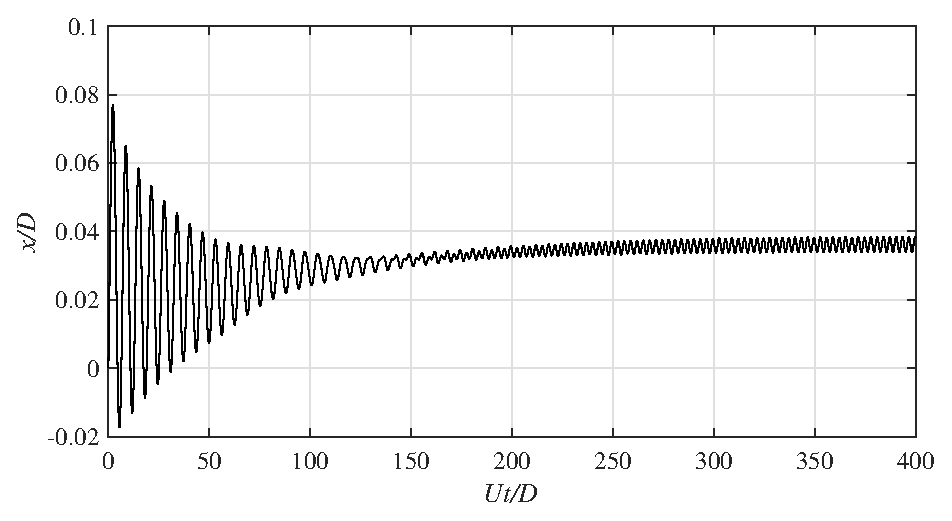
\includegraphics[width=\linewidth]{images/xdisp1.eps}
        \caption{$x$-component displacement}
     \end{subfigure}
    \begin{subfigure}[b]{0.6\linewidth}
        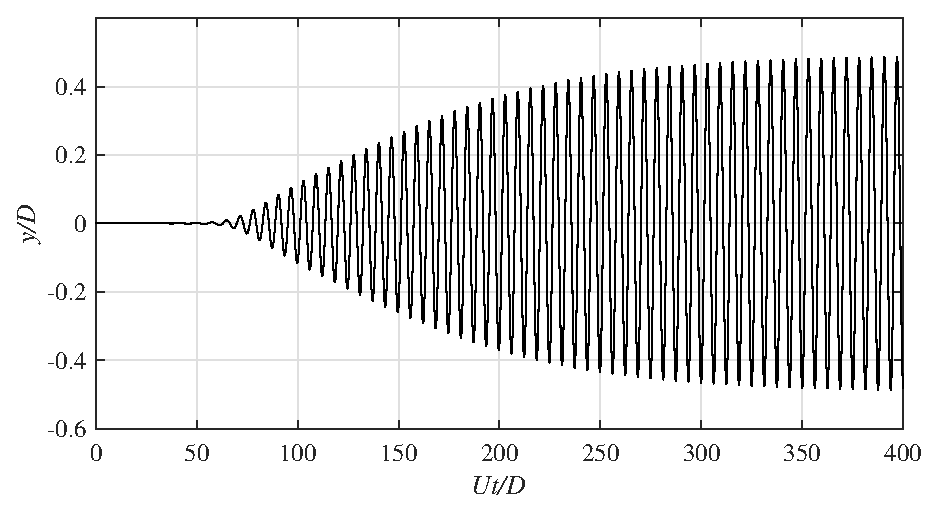
\includegraphics[width=\linewidth]{images/ydisp1.eps}
        \caption{$y$-component displacement}
    \end{subfigure}
      \caption{Time history of the displacement of the rigid circular cylinder}\label{results1}
\end{figure}

\section{VIV of a elastic circular cylinder}

\subsection{Case setup introduction}

This tutorial simulates the vortex-induced vibration of a three-dimensional (3D) elastic circular cylinder of the dimensions 10$D$ in length and $D$ in diameter. The cylinder can be viewed as an elastic beam with tension, compression, bending and torsional deformation capabilities. Without loss of generality, we divide the cylinder into twenty segments so that each segment has the length of $0.5D$. Both two ends of the cylinder are assigned with a fixed support. The cylinder is also assigned with a zero structural damping and low non-dimensional mass to encourage high-amplitude oscillations. Simulations are carried out on a 3D O-block mesh with a outer diameter $15D$ and $80\times80\times20$ finite volume cells. Grid points are uniform distributed in circumferential and spanwise directions, while in radical direction, the grid spacing follows from an exponential distribution with an exponential coefficient of 1.0478. 

\subsection{Procedure}

The detailed procedures of this tutorial are identical to the previous one, as well as most of the case files in these two tutorials. We now demonstrate the remaining differences between them. In the file blockMeshDict, the block entry now takes the form 

\begin{lstlisting}
blocks
(
    hex (1 4 10 7 0 5 11 6) (22 20 80) simpleGrading (1 1 40)
    hex (3 1 7 9 2 0 6 8) (22 20 80) simpleGrading (1 1 40)
    hex (4 3 9 10 5 2 8 11) (36 20 80) simpleGrading (1 1 40)
);
\end{lstlisting}

\noindent The types of the `front' and `back' patches are changed from empty to cyclic.

\begin{lstlisting}
    front
    {
        type cyclic;
        neighbourPatch back;
        faces
        (
            (0 5 4 1)
            (4 5 2 3)
            (3 2 0 1)
        );
    }
    back
    {
        type cyclic;
        neighbourPatch front;
        faces
        (
            (6 11 10 7)
            (10 11 8 9)
            (9 8 6 7)
        );
    }
\end{lstlisting}

\noindent In the file constant/dynamicMeshDict, the keyword `nNode' now takes the value of 21 considering the cylinder is divided into 20 segments. Meanwhile, the entry `length' (which takes a list of scalars as an input) now writes

\begin{lstlisting}
// Select "sixDoFElasticBodyMotion" for 6DoFs beams
motionSolver    sixDoFElasticBodyMotion;

// Number of nodes (an integer larger than 2) on the beam
nNode 21;

// Length of element segments (the number of elements should equal to $nNode minus 1)
length 20{0.5}
\end{lstlisting}

\noindent  Accordingly, the shape of the first mode, in which the cylinder undergoes a bending deflection in the $XZ$ plane, is expressed as 

\begin{lstlisting}
// The first mode (a list of six-component vectors for 6DoFs beams)
mode1 List<vector6D>
21
(
((0.000000 0 0) (0 0.000000 0))
((0.024472 0 0) (0 0.097081 0))
((0.095492 0 0) (0 0.184658 0))
((0.206107 0 0) (0 0.254160 0))
((0.345492 0 0) (0 0.298783 0))
((0.500000 0 0) (0 0.314159 0))
((0.654508 0 0) (0 0.298783 0))
((0.793893 0 0) (0 0.254160 0))
((0.904508 0 0) (0 0.184658 0))
((0.975528 0 0) (0 0.097081 0))
((1.000000 0 0) (0 0.000000 0))
((0.975528 0 0) (0 -0.097081 0))
((0.904508 0 0) (0 -0.184658 0))
((0.793893 0 0) (0 -0.254160 0))
((0.654508 0 0) (0 -0.298783 0))
((0.500000 0 0) (0 -0.314159 0))
((0.345492 0 0) (0 -0.298783 0))
((0.206107 0 0) (0 -0.254160 0))
((0.095492 0 0) (0 -0.184658 0))
((0.024472 0 0) (0 -0.097081 0))
((0.000000 0 0) (0 0.000000 0))
);
\end{lstlisting}

\noindent Similarly, the shape of the second mode takes the form

\begin{lstlisting}
// The second mode (a list of six-component vectors for 6DoFs beams)
mode2 List<vector6D>
21
(
((0 0.000000 0) (0.000000 0 0))
((0 0.024472 0) (-0.097081 0 0))
((0 0.095492 0) (-0.184658 0 0))
((0 0.206107 0) (-0.254160 0 0))
((0 0.345492 0) (-0.298783 0 0))
((0 0.500000 0) (-0.314159 0 0))
((0 0.654508 0) (-0.298783 0 0))
((0 0.793893 0) (-0.254160 0 0))
((0 0.904508 0) (-0.184658 0 0))
((0 0.975528 0) (-0.097081 0 0))
((0 1.000000 0) (0.000000 0 0))
((0 0.975528 0) (0.097081 0 0))
((0 0.904508 0) (0.184658 0 0))
((0 0.793893 0) (0.254160 0 0))
((0 0.654508 0) (0.298783 0 0))
((0 0.500000 0) (0.314159 0 0))
((0 0.345492 0) (0.298783 0 0))
((0 0.206107 0) (0.254160 0 0))
((0 0.095492 0) (0.184658 0 0))
((0 0.024472 0) (0.097081 0 0))
((0 0.000000 0) (0.000000 0 0))
);
\end{lstlisting}

Finally, one can quickly run this tutorial by executing the Allrun command in the terminal as shown below

\begin{quote}
\begin{verbatim}
$ ./Allrun
\end{verbatim}
\end{quote}

\subsection{Results}

Figure \ref{results2} plots the time history of the displacement of the elastic circular cylinder at its mid-point.

\begin{figure}[H]
\centering
    \begin{subfigure}[b]{0.6\linewidth}
        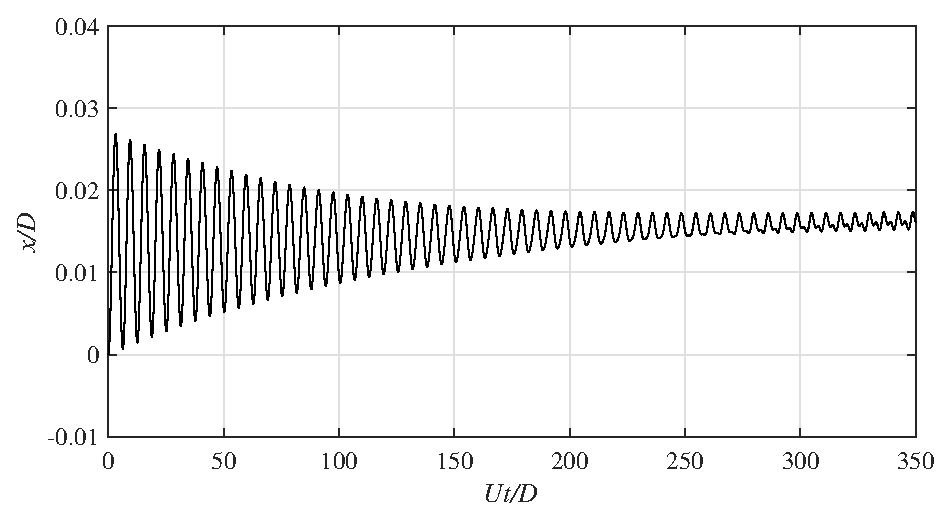
\includegraphics[width=\linewidth]{images/xdisp2.eps}
        \caption{$x$-component displacement}
     \end{subfigure}
    \begin{subfigure}[b]{0.6\linewidth}
        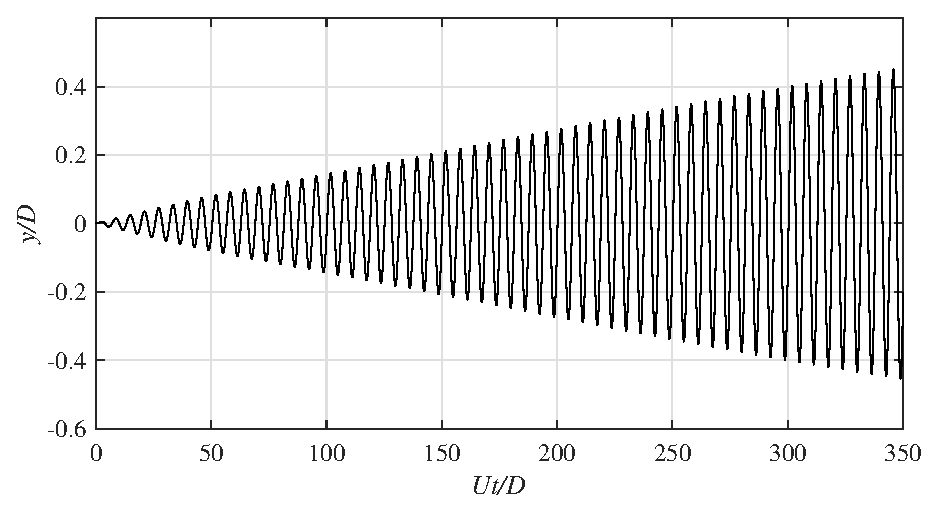
\includegraphics[width=\linewidth]{images/ydisp2.eps}
        \caption{$y$-component displacement}
    \end{subfigure}
      \caption{Time history of the displacement of the elastic circular cylinder at its mid-point}\label{results2}
\end{figure}